\section{Problemanalyse}
I denne moderne tid, hvor massive mængder af kommunikation foregår over internettet, har det aldrig været nemmere at kommunikere med andre mennesker i verdenen. Netop på grund af denne store mængde og tilgængeligheden af digital kommunikation, er internettet også overvåget i en historisk uset grad. Dette betyder, at kommunikation aldrig har været nemmere, men heller aldrig før har så mange kunne følge med i samtaler, der ikke vedrører dem.\cite{Adgang_PersonligeData} På trods af dette er de teknologiske muligheder for at skjule kommunikation store, men ikke realiseret til deres fulde potentiale. Overvågningen bliver også skubbet til det yderste, og som et led i at undgå en fremtid med totalitære styrer, der besidder al information, kræves et modspil, som kan genvinde friheden på internettet, og dermed friheden i verdenen. 
Den største kommunikationsplatform i verden på nuværende tidspunkt er, det sociale netværk Facebook, med sine 2,129 milliarder månedlige aktive brugere gennemsnitligt i løbet af 4. kvartal 2017.\cite{FacebookStat} Facebook har med sin enorme brugerbase, vakt en sådan interesse fra diverse regeringer, bl.a. omhandlede agtindsigt i brugerdata. En rapport fra Facebook selv udgivet i 2013, beskrev blandandet hvordan de i mindst 80 procent af tilfældene, hvor USAs regering efterspørger brugerdata, også har måttet være nød til at udleveret disse data.\cite{PolitikenFacebook} Andre store sociale netværk som Twitter og LinkedIn, har rapporteret lignede forhold.\cite{PolitikenFacebook}

Dette leder cidere frem til den initierende problemformulering:
\begin{mdframed}[linewidth=0pt,backgroundcolor=lightgray!20,innertopmargin = 0.2cm,innerbottommargin = 0.2cm]
    \textit{Hvordan kan man lave en sikker kommunikationsplatform uden at kommunikationen bliver udsat for overvågning fra uvedkommende?}
\end{mdframed}

\newpage
\subsection{Sikker kommunikation}
Der vil i dette afsnit blive kigget på hvad det vil sige at kommunikere sikkert, både i levering, men også i håndteringen af kommunikationen. Tilsidst vil der blive konkluderet et grundlag for foretagelse af sikker kommunikation.

\subsubsection{Kryptologi}
De fleste forbinder moderne IT-sikkerhed med avanceret krypteringsalgoritmer. Selvom dette er en vigtig del af IT-sikkerhed, er det dog ikke den eneste måde at sikre kommunikation på. Under emnet kryptologi, som omhandler alle former for hemmelig kommunikation, er kryptografi kun en del af emnet. Et andet vigtigt koncept som også dækker er steganografi, der videre vil blive diskuteret i næste afsnit. Den førnævnte algoritmebaseret sikring af data falder ind under kryptografi. Eksempler på disse spænder fra den simpleste alfabet skiftende algoritme, f.eks. ét bogstav skift til højre, og videre til moderne hashing algoritmer. Fælles for anvendelsen af alle disse er dog, at det tydeligt viser en intention om at hemmeligholde indholdet. Hermed kan selve krypteringen gøre beskeden mistænkelig, da information af lav værdi ikke ville være besværet værd.

\subsubsection{Steganografi}
Som nævnt i indledningen, består emnet kryptologi af flere underkategorier. Den kategori der vil blive fokuseret på her, er steganografi. Steganografi omhandler metoder til at skjule selve eksistensen af en given besked, i stedet for at gøre indeholdet ulæseligt, som er hvad kryptografi gør.\cite{MeningOfSteganografi} Et eksempel på beskeder der er sikret med steganografi, kunne være de hemmelige tegn og signaler, også ofte brugt af spioner i film. Et tilsyneladende tilfældigt symbol på et umiddelbart ligegyldigt sted, men blot en af de mange forskellige ting som kunne sende en besked sikkert frem. Alt dette vil foregå imens ingen andre vil opdage, at der overhovedet var en form for kommunikation. Udenfor fiktionens verden findes der dog også nogle eksempler på grupper, som har udviklet systemer baseret på steganografi til at kommunikere internt.
\begin{figure}[H]
    \begin{subfigure}{0.5\textwidth}
    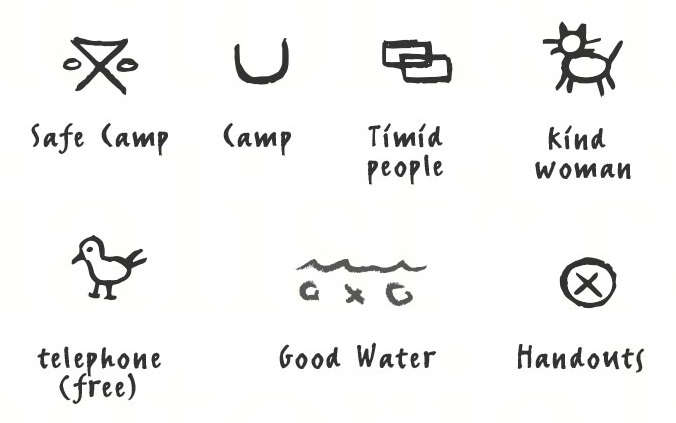
\includegraphics[width=0.9\linewidth, height=5cm]{Projectdoc/Problemanalyse/Illustrationer/hobo.jpg} 
    \caption{The Hobo Code}
    \label{fig:hobocode}
    \end{subfigure}
    \begin{subfigure}{0.5\textwidth}
    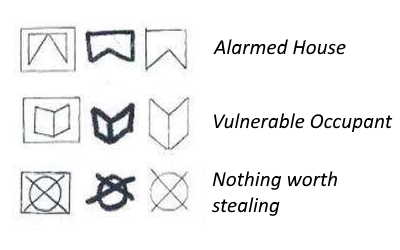
\includegraphics[width=0.9\linewidth, height=5cm]{Projectdoc/Problemanalyse/Illustrationer/da-code.png}
    \caption{Da Pinchi Code / The Burglars Code}
    \label{fig:burglarscode}
    \end{subfigure}
    \caption{To af de legendariske steganografi metoder}
    \label{fig:legendscode}
\end{figure}
Et kendt eksempel på sådan et steganografisk system kunne være "The Hobo Code [Se figur: \ref{fig:hobocode}]", et system kendt, og anvendt, af hjemløse til at hjælpe hinanden med deres overlevelse\cite{TheHoboCode}. Disse beskeder er aldrig rigtigt blevet dateret, og ingen i dag kender derfor deres præcise oprindelse, men det vides dog stadig at dette steganografiske system har været anvendt i flere århundrede.\\ 
Foruden videnen om metodens eksistens gennem årene, vides også at der findes flere andre ligende afarter af denne kendte kode, såsom den nytidiske "Da Pinchi Code [Se figur: \ref{fig:burglarscode}]". Denne kode bliver alment anvendt af konstruktions arbejdere, men siges også, efter historier, at have været anvendt af indbrudstyve eller andre kriminelle.\cite{DaPinchiCode} At lave sikre systemer handler dog ikke kun om den underlæggende teori. Brugerne af systemet kan også lave fejl, eller bruge systemet på ikke tiltænkte måder, som potentielt kunne skade systemet, eller brugerne, som en helhed. Derfor vil der i det næste afsnit diskuteres en sådan brugerbaseret problematik. 

\subsubsection{Brugeren som sikkerhedsbrist}
\label{Brugeren_som_sikkerhedsbrist}
I dag forsøger mange at bibeholde, hvad der for dem synes at være, sikker eller hemmelig kommunikation via diverse tjenester. For nogle er disse tjenester dog mere sikre end hos andre. Som et eksempel vil de fleste private computerbrugere, nok mene at deres generelle email er forholdsvis sikker, men deres arbejdsplads deler muligvis ikke samme overbevisning. Dette var f.eks. tilfældet hos Hillary Clintons email-skandale tilbage i 2015-2016.\cite{Hillary_Email_History} Hillary Clinton havde oprettet sin egen mailserver til håndtering af alle hendes mails, dog mener flere, blandet andet FBI, at denne handling har været en "ekstremt uforsigtigt" håndtering af hendes fortrolighed. Trods Hillarys skandale menes dog ikke at et større sikkerhedsbrud har fundet sted, men Hillary har stadig som bruger mindsket den tilgængelige sikkerhed, i følge FBI, da de mener at hun fejlagtigt har misbrugt det vante system.\cite{Hillary_Email_skandale} Det efterfølgende afsnit vil danne overblik over de vigtigste elementer af sikker kommunikation.

\subsubsection{Grundlaget for sikker kommunikation}
I dag forsøger folk ved alle tænkelige metoder at kryptere forbindelser på nettet, men da kryptering er kendt og synligt, vil det derfor på et eller andet tidspunkt blive, eller være forsøgt, brudt. Steganografiske metoder har til gengæld alle den vigtige egenskab, at ikke alle vil ligge mærke til dem, selvom de befinder sig lige foran dem. Steganografiens egenskaber kan sammen med de sociale mediers endeløse strøm af indhold, fungere som et ekstra lag af sikkerhed. Udover kommunikationens skjulte eksistens, vil den kommunikation være at finde blandt milliarder af uskyldige indlæg.\\
En effektiv implementation af dette, kunne endda sikre kommunikation imellem stridende lande, hvor sikker og åben kommunikation ikke er en selvfølge.
Dog skal man også, for en endelig metode, have i tanke, at jo mere frihed man giver en bruger, jo større er risikoen for, at brugeren anvender systemet på en ikke tiltænkt, eller ligefrem uforsvarlig måde.
\\\\
I det næste afsnit vil nogle udvalgte kommunikationsplatforme blive analyseret baseret på netop disse kriterier.
\newpage
\subsection{Sikring af kommunikationsplatforme}
\label{kommunikationsplatforme}
For at undersøge hvordan moderne kommunikationsplatforme sikrer deres brugere vil to af de største, Facebooks Messenger og WhatsApp, blive diskuteret. I Messenger appen findes en indstilling til at lave en End to End krypteret chat med én anden person. Hvis man ikke kender til funktionens eksistens, så opdager man den måske ikke [Se appendix \ref{appendix:facebookchat} for en forløbsgennemgang]. WhatsApp har derimod End to End kryptering aktiveret som standard, også for gruppe chats. Forskellen ligger her i, at den informerede bruger kan kommunikere sikkert over begge platforme, men dette kræver dog, at den enkelte bruger selv aktiverer sikkerheden. Dette medfører i praksis, at en del af bruger basen er mindre sikret kun grundet manglen på kendskab til denne sikkerhedsfunktion. Hvorfor er denne kryptering ikke standard på Messenger, når Facebook også ejer WhatsApp\cite{Facebook_WhatsApp_Merger}, hvor det er standard? Dette kunne være for at undgå potentielle problemer med blokering i visse lande\cite{Facebook_security_features}, så som sagen med blokeringen af WhatsApp i Brasilien [Forklares i afsnit \ref{politisk_censur}]. Samtidigt kunne de ukrypterede chats over Messenger, principielt, være materiale for deres individuelt tilpassede reklamer.
\\
Herefter vil det være naturligt, at betragte WhatsApp som det rigtige valg til privat kommunikation. Problemet med den konklusion er dog tofoldig. Først kan nævnes at man i nogle lande kunne blive mistænkt for at gemme på noget, kun fordi man bruger en platform med bedre sikkerhed end Messenger. Dette er naturligvis aldrig en god ting. For det andet, bør man også overveje hvordan resten af systemet fungerer. Selvom WhatsApp bruger End to End kryptering så har systemet et antal problemer i følge "Electronic Frontier Foundation"\cite{WhatsApp_Security_Concerns}. Ét af disse problemer er et sikkerhedshul som ligger i muligheden for, at lave backups i Google Drev. Denne feature gør det nemt at skifte til et nyt device. Problemet ligger i det faktum at disse backups ikke er krypteret. En konsekvens af dette er, at mange brugers chats kan kompromitteres af én brugers ukrypterede cloud backup. Hermed kommer den enkelte brugers valg af sikkerhedsindstillinger til at påvirke andre brugere, som ikke kan gøre noget for at beskytte sig imod dette problem.
\\
Det kan derfor konkluderes at med to af de mest brugte kommunikationsplatforme, så kan bevidsthed fra den enkelte brugers part gøre en forskel, men også at andre brugers mangel på samme også kan have en negativ indflydelse på det velvidende indvid. Individets sikkerhed på en kommunikationsplatform burde ikke være afhængigt af andre brugeres valg af indstillinger.
\newpage
\subsection{Overvågning af kommunikation på nettet}
Der vil i dette afsnit blive kigget på hvordan og hvorfor der foregår overvågning og censur på internettet.

\subsubsection{Politisk censur og manipulation}
\label{politisk_censur}
I 2015 fandt Freedom House, som er en uafhængig frihedskæmpende organisation, frem til, at 15 regeringer ud af de 65 undersøgte, havde begrænset befolkningens adgang til diverse sociale medier.\cite{FreedomHouseRapport2016} Tendensen havde i 2016 vokset sig til 24 regeringer.\cite{FreedomHouseRapport2016} Brasilien og Tyrkiet endte 2016's undersøgelse med, at blive to af de mest bemærkelsesværdige lande, da de begge gik et betydeligt skidt tilbage på deres respektive frihedsskalaer, netop på grund af deres magtanvendelse overfor diverse sociale medier. Brasilien gik fra kategorien "Free" til "Partly Free", da brasilianske domstole indførte en midlertidig blokering af opkald- og tekstkommunikations tjenesten WhatsApp. WhatsApp nægtede nemlig at udlevere brugerdata til bevismateriale. Tyrkiet gik fra kategorien "Partly Free" til "Not Free" efter masseblokeringer af diverse sociale medier, og efterfølgende forfølgelse af borgere, der kritiserede Tyrkiets regering.\cite{FreedomHouseRapport2016}

Det kan virke som om at de sociale medier kun er til befolkningens fordel, med eksempler på organisering af store demonstrationer og muligheden for at dele beretninger om uretfærdighed fra hele kloden. Virkeligheden er dog at regeringerne lytter med. Regeringer er blevet bedre til at manipulere og sprede deres politiske agenda på de sociale medier end borgerne og aktivisterne.\cite{SocialHelpDictators} Det ses blandt andet i Freedom Houses rapport fra 2017, som fandt mindst 18 regeringer der, med hjælp af sociale medier, aktivt har spredt misinformation der manipulerede med valgenes valg, heriblandt det demokratiske land USA.\cite{FreedomHouseRapport2017} Et af de eksempler på hvorfor USA er at finde på listen over disse land, er blandt andet Trumps kampagne og deres brug af Cambridge Analyticas tvivlsomme brug af data [Ses nærmere i afsnit \ref{national_privatliv}].\cite{Cambridge_Analytica_Zuckerberg}
Dertil kommer forgangsprogrammer som den amerikanske efterretningtjeneste NSAs PRISM, som tillader dommerkendelsesløs aflytning af blandt andet email, netopkald og kommunikation over sociale medier,\cite{PRISM} der er med til at skubbe grænserne for regeringers kontrollering af deres befolkning. Politisk censur og manipulation af internettet hører ikke blot diktatorer til, men er et globalt fænomen der ikke viser de store tegn på at begrænse sig.\cite{FreedomHouseRapport2017}

\subsubsection{National sikkerhed kontra privatliv}
\label{national_privatliv}
Når privatlivets fred diskuteres kommer to grundlæggende holdninger ofte op. De to yderpunkter er, "Overvågning er ikke et problem hvis du ikke har noget at skjule" og "Ingen skal have ret til at vide hvad jeg laver". Situationen er så at begge yderpunkter har problemer. Hvis individet f.eks. var garanteret at ingen agentur kunne overvåge, undersøge, eller blot spørge til, aktiviteter så ville det ikke være muligt at beskytte almene borgere mod kriminalitet og terror. På den anden side vil et samfund i den anden ende af spektrummet også være i stand til at bruge informationen imod borgernes interesse. 
Et eksempel på denne form for misbrug af data er sagen med Cambridge Analytica, som har benyttet data fra 87 millioner Facebook brugere til bl.a. at hjælpe Trumps valgkampagne i 2016.\cite{Cambridge_Analytica_Zuckerberg} Denne type anvendelse af data kunne have omfattende konsekvenser for demokratiets grundlag, hvis enhver siddende regering kunne bruge deres borgeres information i lignende Big Data baseret valgkampanger. 

Et andet eksempel på konflikten mellem national sikkerhed og privatlivets fred er bagdøre til krypterede systemer. På den ene side ville denne bagdør blive brugt af regeringer til at fremme efterforskningen af kriminelle. På den anden side kan sådanne bagdøre også anvendes af kriminelle for finansielle gevinster eller af regeringer som vil undertrykke deres befolkninger. FBI og Apple har været i netop sådanne situationer hvor Apple ikke har ville lave en generel bagdør til FBI. Dette valg traf de for at beskytte deres brugere.\cite{FBI/Apple_encryption}

Essensen er, at de fleste mennesker er enige om, at samfundet burde have sikkerhedsforanstaltninger imod kriminalitet og terrorisme. Samtidigt vil borgere gerne have en del privatliv. Både fordi det er ubehageligt at blive overvåget i alle aspekter af ens liv, men også fordi der er potentielt store konsekvenser, hvis ikke dette er tilfældet.

% Det egentlige spørgsmål kommer tilbage til: Hvor meget overvågning er for meget? Dette projekt vil tage udgangspunkt i den overbevisning at der ikke ønskes et samfund hvor man ikke har ret til et privatliv. 

% Udviklingen har igennem længere tid været sådan, at regeringer har fundet nye måder at overvåge befolkningen på, og efter noget tid, er det blevet fastslået ved lov, i hvilken grad, og i hvilke tilfælde, at denne type overvågning skal være lovlig. I de seneste år har udviklingen af teknologi dog været meget hurtigere end retssystemet. Det har derfor været svært at regulere disse nye teknologier på passende vis. Problemet er dog mere omfattende når stater uden veletableret retssystemer betragtes. I disse stater kan regeringer bruge disse nye teknologier til at fremme deres egne formål. Borgerne i disse stater har så adopteret metoder til at undgå overvågning, så som VPN tjenester og TOR netværket. Regeringer kan så som modsvar blokere VPN tjenester i en stor udstrækning. At blokere borgere fra at bruge TOR netværket er dog ikke lige til, da al trafikken er krypteret og tager tilfældige veje igennem netværket. Problemet ved dette er, at meget store mængder trafik kan blive betragtet som værende forsøg på hemmelig kommunikation.